%% LyX 2.0.3 created this file.  For more info, see http://www.lyx.org/.
%% Do not edit unless you really know what you are doing.
\documentclass[twoside,english]{paper}
\usepackage{lmodern}
\renewcommand{\ttdefault}{lmodern}
\usepackage[T1]{fontenc}
\usepackage[latin9]{inputenc}
\usepackage[a4paper]{geometry}
\geometry{verbose,tmargin=3cm,bmargin=2.5cm,lmargin=2cm,rmargin=2cm}
\usepackage{color}
\usepackage{babel}
\usepackage{float}
\usepackage{bm}
\usepackage{amsthm}
\usepackage{amsmath}
\usepackage{amssymb}
\usepackage{graphicx}
\usepackage{esint}
\usepackage[unicode=true,pdfusetitle,
 bookmarks=true,bookmarksnumbered=false,bookmarksopen=false,
 breaklinks=false,pdfborder={0 0 0},backref=false,colorlinks=false]
 {hyperref}
\usepackage{breakurl}
\usepackage{makeidx}

\makeatletter

%%%%%%%%%%%%%%%%%%%%%%%%%%%%%% LyX specific LaTeX commands.
%% Because html converters don't know tabularnewline
\providecommand{\tabularnewline}{\\}

%%%%%%%%%%%%%%%%%%%%%%%%%%%%%% Textclass specific LaTeX commands.
\numberwithin{equation}{section}
\numberwithin{figure}{section}

%%%%%%%%%%%%%%%%%%%%%%%%%%%%%% User specified LaTeX commands.
\usepackage{babel}

\@ifundefined{showcaptionsetup}{}{%
 \PassOptionsToPackage{caption=false}{subfig}}
\usepackage{subfig}
\makeatother

\usepackage{listings}


\begin{document}

\title{Generalised parton distributions}

\author{Valerio Bertone}

\tableofcontents{}

\section{Introduction}

In this set of notes I collect the technical aspects concerning
generalised parton distributions (GPDs). Since the computation GPDs
introduces new kinds of convolution integrals, a strategy aimed at
optimising the numerics needs to be devised.

\section{Evolution equation}

The evolution equation for GPDs reads:
\begin{equation}\label{eq:eveq}
\mu^2\frac{d}{d\mu^2}f(x,\xi) = \int_{-\infty}^{+\infty}\frac{dx'}{\left|2\xi\right|}\mathbb{P}\left(\frac{x}{\xi},\frac{x'}{\xi}\right)f(x',\xi)\,.
\end{equation}
In general, the GPD $f$ and the evolution kernel $\mathbb{P}$ should
be respectively interpreted as a vector and a matrix in flavour
space. However, for now, we will just be concerned with the integral
in the r.h.s. of Eq.~(\ref{eq:eveq}) regardless of the flavour
structure.

The support of the evolution kernel
$\mathbb{P}\left(\frac{x}{\xi},\frac{x'}{\xi}\right)$ is shown in
Fig.~\ref{fig:GPDIntDomain}.
\begin{figure}[h]
  \begin{centering}
    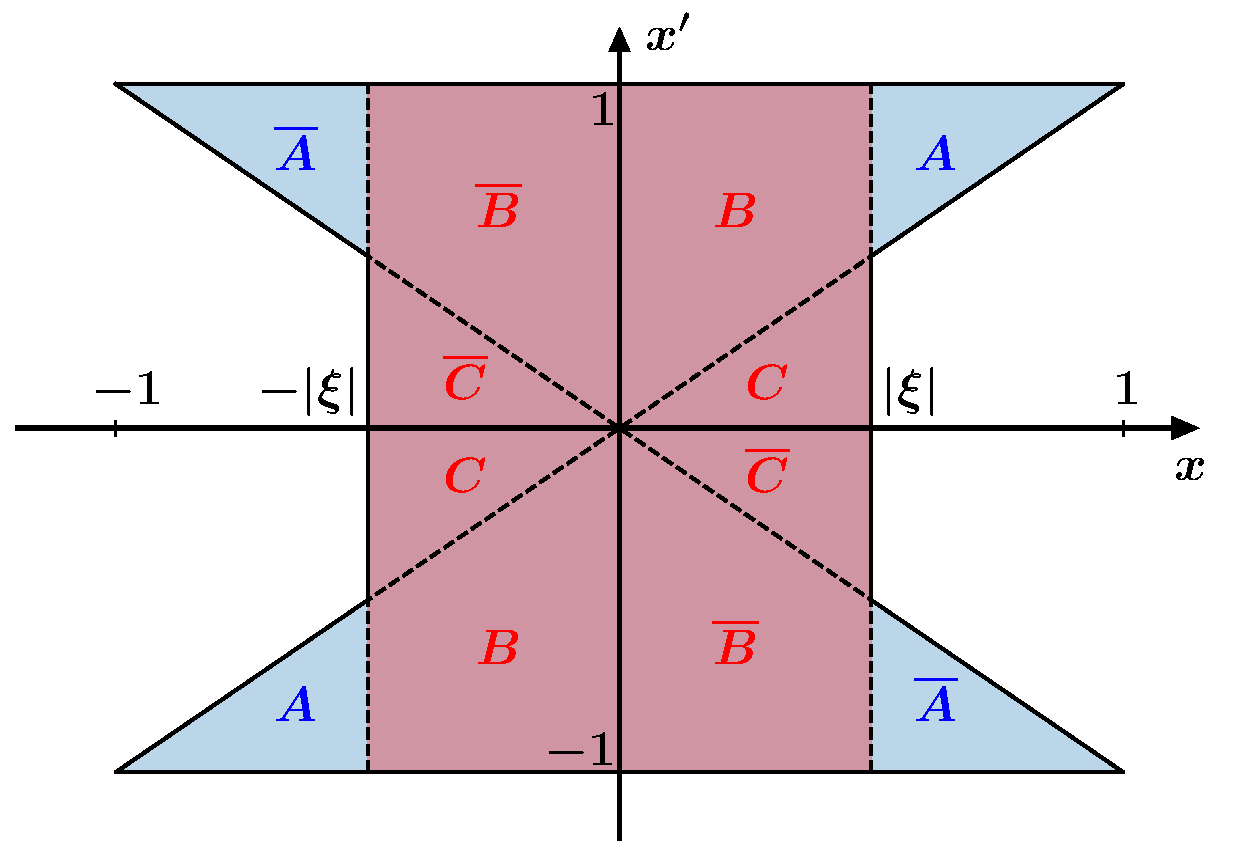
\includegraphics[width=0.7\textwidth]{plots/GPDIntDomain}
    \caption{Support domain of the evolution kernel
      $\mathbb{P}\left(\frac{x}{\xi},\frac{x'}{\xi}\right)$.\label{fig:GPDIntDomain}}
  \end{centering}
\end{figure}
The Knowledge of the support region of the evolution kernel allows us
to rearrange Eq.~(\ref{eq:eveq}) as follows:
\begin{equation}
\displaystyle\mu^2\frac{d}{d\mu^2}f(\pm x,\xi) =\int_{b(x)}^{1}\frac{dx'}{x'}\left[\frac{x'}{\left|2\xi\right|}\mathbb{P}\left(\pm \frac{x}{\xi},\frac{x'}{\xi}\right)f(x',\xi)+\frac{x'}{\left|2\xi\right|}\mathbb{P}\left(\mp \frac{x}{\xi},\frac{x'}{\xi}\right)f(-x',\xi)\right]\,,
\end{equation}
with:
\begin{equation}\label{eq:lowintb}
b(x) = |x|\theta\left(\left|\frac{x}{\xi}\right|-1\right)\,,
\end{equation}
and where we have used the symmetry property of the evolution kernels:
$\mathbb{P}(y,y')=\mathbb{P}(-y,-y')$. In the unpolarised case, it is
useful to define:\footnote{Notice the seemingly unusual fact that
  $f^{+}$ is defined as difference and $f^{-}$ as sum of GPDs computed
  at opposite values of $x$. This can be understood from the fact
  that, in the forward limit, $f(-x)= -\overline{f}(x)$, \textit{i.e.}
  the PDF of a quark computed at $-x$ equals the PDF of the
  corresponding antiquark computed at $x$ with opposite sign. The
  opposite sign is absent in the longitudinally polarised case.}
\begin{equation}\label{eq:pmdef}
\begin{array}{rcl}
\displaystyle f^{\pm}(x,\xi) &=&\displaystyle  f(x,\xi) \mp
                       f(-x,\xi)\,,\\
\\
\displaystyle \mathbb{P}^{\pm}(y,y') &=&\displaystyle  \mathbb{P}(y,y') \mp \mathbb{P}(-y,y')\,,
\end{array}
\end{equation}
so that the evolution equation for $f^{\pm}$ reads:
\begin{equation}\label{eq:eveq2}
\displaystyle\mu^2\frac{d}{d\mu^2}f^{\pm}(x,\xi) = \int_{b(x)}^{1}\frac{dx'}{x'}\frac{x'}{\left|2\xi\right|}
                                                         \mathbb{P}^{\pm}\left(\frac{x}{\xi},\frac{x'}{\xi}\right)f^{\pm}(x',\xi)\,.
\end{equation}
The $f^{\pm}$ distributions can be regarded as the GPD analogous of
the $\pm$ forward distributions that can then be used to construct the
usual singlet and non-singlet distributions in the QCD evolution
basis. This uniquely determines the flavour structure of the evolution
kernels $\mathbb{P}^{\pm}$.

It is relevant to observe that the presence of the $\theta$-function
in the lower integration bound $b$, Eq.~(\ref{eq:lowintb}), is such
that for $|x|>|\xi|$ the evolution equation has the exact form of the
DGLAP evolution equation which corresponds to integrating over the
blue regions in Fig.~\ref{fig:GPDIntDomain} (DGLAP region,
henceforth). Conversely, for $|x|\leq|\xi|$ the lower integration
bound becomes zero and the evolution equation assumes the form of the
so-called ERBL equation that describes the evolution of meson
distribution amplitudes (DAs). This corresponds to integrating over
the red region (ERBL region, henceforth). Crucially, in the limits
$\xi\rightarrow 0$ and $\xi\rightarrow \pm1$ Eq.~(\ref{eq:eveq2})
needs to recover the DGLAP and ERBL equations, respectively.

GPD anomalous dimensions are generally tricky to integrate numerically
because of the intricate support. In order to simplify the integration
procedure, we can decompose the anomalous dimensions using the labels
given in Fig.~\ref{fig:GPDIntDomain} as a guide:
\begin{equation}
\begin{array}{rcl}
\displaystyle\mathbb{P}(y,y')&=&\displaystyle
  \theta(y')\\
\\
&\times&\Big[\theta(y-1)\theta(y'-y)\mathbb{P}_A(y,y')+\theta(1-y)
  \theta(y'-y)\mathbb{P}_B(y,y') +\theta(1-y)
  \theta(y-y')\mathbb{P}_C(y,y')\\
\\
&+&\displaystyle \theta(-y-1)\theta(y+y')\mathbb{P}_{\overline{A}}(y,y')+\theta(1+y)
  \theta(y+y')\mathbb{P}_{\overline{B}} (y,y') +\theta(1+y)
  \theta(-y'-y)\mathbb{P}_{\overline{C}} (y,y')\Big]\\
\\
&+&\displaystyle \theta(-y')\\
\\
&\times&\displaystyle\Big[\theta(y-1)\theta(-y-y')\mathbb{P}_{\overline{A}}(y,y')+\theta(1-y)
  \theta(-y-y')\mathbb{P}_{\overline{B}} (y,y') +\theta(1-y)
  \theta(y'+y)\mathbb{P}_{\overline{C}} (y,y')\\
\\
&+&\displaystyle\theta(-y-1)\theta(-y'+y)\mathbb{P}_A(y,y')+\theta(1+y)
  \theta(-y'+y)\mathbb{P}_B(y,y') +\theta(1+y)
  \theta(-y+y')\mathbb{P}_C(y,y')\Big]\,,
\end{array}
\end{equation}
where the functions $\mathbb{P}_I$ and $\mathbb{P}_{\overline{I}}$,
with $I=A,B,C$, are defined on the respective regions in
Fig.~\ref{fig:GPDIntDomain}.\footnote{Note that $\mathbb{P}_I(y,y')$
  and $\mathbb{P}_{\overline{I}}(y,y')$ are not required to be
  symmetric upon the transformation
  $(y \rightarrow -y, y' \rightarrow -y')$.}  Next, we take the
combinations given in Eq.~(\ref{eq:pmdef}) relevant to implement the
evolution equation in Eq.~(\ref{eq:eveq2}). By doing this, one
obtains:
\begin{equation}\label{eq:DGLAPsuitable}
  \mathbb{P}^\pm(y,y')=\theta(y-1)\mathbb{P}_A^\pm(y,y')+\theta(1-y)
  \left[\theta(y'-y)\mathbb{P}_B^\pm(y,y') +
    \theta(y-y')\mathbb{P}_C^\pm(y,y')\right]\,,
\end{equation}
where we have defined:
\begin{equation}
\mathbb{P}_I^{\pm}(y,y') = \mathbb{P}_I(y,y')\mp
\mathbb{P}_{\overline{I}}(-y,y')\,,
\end{equation}
and omitted all the irrelevant/redundant terms and factors for the
computation of the integral in the r.h.s. of
Eq.~(\ref{eq:eveq2}). From Eq.~(\ref{eq:DGLAPsuitable}), it should be
clear that the anomalous dimension $\mathbb{P}_A^\pm$ is responsible
for the evolution in the DGLAP region while $\mathbb{P}_B^\pm$ and
$\mathbb{P}_C^\pm$ are responsible for the evolution in the ERBL
region. The latter observation suggests that $\mathbb{P}_B^\pm$ and
$\mathbb{P}_C^\pm$ are related. The relation can easily be established
by observing that the general structure of the ERBL anomalous
dimensions is:
\begin{equation}
V^{\rm ERBL}(y,y')=\theta(y'-y)F(y,y')+\theta(y-y')F(-y,-y')\,,
\end{equation}
which immediately implies that:
\begin{equation}
\mathbb{P}_C^\pm(y,y')=\mathbb{P}_B^\pm(-y,-y')\,.
\end{equation}
Finally, one finds that a convenient decomposition for the anomalous
dimension in Eq.~(\ref{eq:eveq2}) is:
\begin{equation}
\mathbb{P}^\pm(y,y')=\theta(y-1)\mathbb{P}_A^\pm(y,y')+\theta(1-y)
  \left[\theta(y'-y)\mathbb{P}_B^\pm(y,y') +
  \theta(y-y')\mathbb{P}_B^\pm(-y,-y')\right]\,.
\end{equation}

Eq.~(\ref{eq:eveq2}) can be further manipulated to make it resemble
the structure of the DGLAP equation as much as possible. To this
purpose, we define the parameter:
\begin{equation}
\kappa(x) = \frac{\xi}{x}\,,
\end{equation}
so that:
\begin{equation}\label{eq:manip}
\frac{x'}{\left|2\xi\right|}
\mathbb{P}_I^{\pm}\left(\pm\frac{x}{\xi}, \pm\frac{x'}{\xi}\right)={\rm sign}(\xi)\frac{1}{2\kappa}
\frac{x'}{x} \mathbb{P}_I^{\pm}\left(\pm\frac{1}{\kappa}, \pm\frac{1}{\kappa}
  \frac{x'}{x}\right)\equiv {\rm sign}(\xi)\mathcal{P}_I^{\pm}\left(\pm\kappa,\frac{x}{x'}\right)\,,
\end{equation}
where the last equality effectively defines the \textit{DGLAP-like}
splitting function:
\begin{equation}\label{eq:DGLAPevk}
  \mathcal{P}_I^{\pm}(\pm\kappa,y) = \frac{1}{2\kappa y}
  \mathbb{P}_I^{\pm}\left(\pm\frac{1}{\kappa}, \pm\frac{1}{\kappa y}\right)\,.
\end{equation}
In the following we will assume $\xi>0$ as, so far, this is the only
experimentally accessible region. This allows us to get rid of
${\rm sign}(\xi)$ in Eq.~(\ref{eq:manip}). In addition, without loss
of generality, we can also restrict ourselves to positive values of
$x$ because negative values can be easily accessed by symmetry using
Eq.~(\ref{eq:pmdef}), \textit{i.e.}
$f^{\pm}(-x,\xi)=\mp f^{\pm}(x,\xi)$. Using the definition in
Eq.~(\ref{eq:DGLAPevk}) in the integral in the r.h.s. of
Eq.~(\ref{eq:eveq2}) and finally performing a change of variable
gives:
\begin{equation}\label{eq:DGLAPforGPDs}
\displaystyle\mu^2\frac{d}{d\mu^2}f^{\pm}(x,\xi)= \int_{b(x)}^{1}\frac{dx'}{x'}\mathcal{P}^{\pm}\left(\kappa, \frac{x}{x'}\right)f^{\pm}\left(x',\xi\right)=\int_{x}^{x/b(x)}\frac{dy}{y}\mathcal{P}^{\pm}\left(\kappa,y\right)f^{\pm}\left(\frac{x}{y},\xi\right)\,,
\end{equation}
with:
\begin{equation}
b(x) = x\,\theta(1-\kappa)\,,
\end{equation}
and:
\begin{equation}\label{eq:DGLAPevkdec}
  \mathcal{P}^{\pm}\left(\kappa,y\right)=\theta(1-\kappa)\mathcal{P}_A^\pm(\kappa,y)+\theta(\kappa-1)
  \left[\theta(1-y)\mathcal{P}_B^\pm(\kappa,y) +
    \theta(y-1)\mathcal{P}_B^\pm(-\kappa,y)\right]\,.
\end{equation}
Plugging Eq.~(\ref{eq:DGLAPevkdec}) into Eq.~(\ref{eq:DGLAPforGPDs}),
one obtains:
\begin{equation}\label{eq:DGLAPforGPDs2}
\begin{array}{rcl}
  \displaystyle\mu^2\frac{d}{d\mu^2}f^{\pm}(x,\xi)&=&\displaystyle
                                                      \int_{x}^{1}\frac{dy}{y}\left[\theta(1-\kappa)\mathcal{P}_A^{\pm}\left(\kappa,y\right)+\theta(\kappa-1)\mathcal{P}_B^{\pm}\left(\kappa,y\right)\right]f^{\pm}\left(\frac{x}{y},\xi\right)\\
  \\
                                                  &+&\displaystyle\theta(\kappa-1)\int_{1}^{\infty}\frac{dy}{y}\mathcal{P}_B^{\pm}\left(-\kappa,
                                                      y\right)f^{\pm}\left(\frac{x}{y},\xi\right)\\
\\
&=&\displaystyle
                                                      \int_{x}^{1}\frac{dy}{y}\left[\theta(1-\kappa)\mathcal{P}_A^{\pm}\left(\kappa,y\right)+\theta(\kappa-1)\left(\mathcal{P}_B^{\pm}\left(\kappa,y\right)-\mathcal{P}_B^{\pm}\left(-\kappa,y\right)\right) \right]f^{\pm}\left(\frac{x}{y},\xi\right)\\
  \\
                                                  &+&\displaystyle\theta(\kappa-1)\int_{x}^{\infty}\frac{dy}{y}\mathcal{P}_B^{\pm}\left(-\kappa,
                                                      y\right)f^{\pm}\left(\frac{x}{y},\xi\right)\,.
\end{array}
\end{equation}
Eq.~(\ref{eq:DGLAPforGPDs2}) has almost the form of a ``standard''
DGLAP equation except for the term in the last line whose integration
range extends between $x$ and $\infty$. This kind of integral can be
handled within APFEL with minor modifications of the integration
strategy and up to a numerical approximation to be assessed. In
addition, one can prove that at one-loop accuracy, the function
$\theta(1-\kappa)\mathcal{P}_A^{\pm}\left(\kappa,y\right)+\theta(\kappa-1)\mathcal{P}_B^{\pm}\left(\kappa,y\right)$
in the integral in the first line is continuos at the point $\kappa=1$
(but not smooth) because:
\begin{equation}\label{eq:continuity}
\mathcal{P}_A^{\pm}\left(1,y\right) = \mathcal{P}_B^{\pm}\left(1,y\right)\,.
\end{equation}

\subsection{On continuity of GPDs}

It is well known that GPDs are required to be continuous at $x=\xi$
for factorisation to be valid~\cite{Radyushkin:1997ki}. It is thus
interesting to consider the consequence of this constraint. To this
end, let us consider the limits of Eq.~(\ref{eq:DGLAPforGPDs2}) for
$x\rightarrow \xi^\pm$, which corresponds to
$\kappa\rightarrow 1^{\pm}$:
\begin{equation}\label{eq:limit1}
\lim_{x\rightarrow
  \xi^+}\displaystyle\mu^2\frac{d}{d\mu^2}f^{\pm}(x,\xi) =
\int_{x}^{1}\frac{dy}{y}\mathcal{P}_B^{\pm}\left(1,y\right)f^{\pm}\left(\frac{x}{y},\xi\right)+\int_{1}^{\infty}\frac{dy}{y}\mathcal{P}_B^{\pm}\left(-1,
                                                      y\right)f^{\pm}\left(\frac{x}{y},\xi\right)\,,
\end{equation}
and:
\begin{equation}\label{eq:limit2}
\lim_{x\rightarrow \xi^-}\displaystyle\mu^2\frac{d}{d\mu^2}f^{\pm}(x,\xi) = \mu^2\frac{d}{d\mu^2}f^{\pm}(\xi,\xi)=\int_{x}^{1}\frac{dy}{y}\mathcal{P}_A^{\pm}\left(1,y\right)f^{\pm}\left(\frac{x}{y},\xi\right)\,.
\end{equation}
Taking the difference between Eqs.~(\ref{eq:limit1})
and~(\ref{eq:limit2}) and using Eq.~(\ref{eq:continuity}) as well as
the continuity of $f^{\rm}$ at $x=\xi$, one finds that:
\begin{equation}
\int_{1}^{\infty}\frac{dy}{y}\mathcal{P}_B^{\pm}\left(-1,
                                                      y\right)f^{\pm}\left(\frac{x}{y},\xi\right)=0\,,
\end{equation}
which has to be valid at any scale and for any $f^{\pm}$. This
immediately implies that:
\begin{equation}\label{eq:contcondition}
\mathcal{P}_B^{\pm}\left(-1, y\right) = 0\,,
\end{equation}
for all values of $y$ and order-by-order in perturbation theory. We
will explicitly verify this constraint when we will discuss the
explicit expressions. Also notice that this constraint, along with
Eq.~(\ref{eq:continuity}), is such that the function
$\theta(1-\kappa)\mathcal{P}_A^{\pm}\left(\kappa,y\right)+\theta(\kappa-1)\left(\mathcal{P}_B^{\pm}\left(\kappa,y\right)-\mathcal{P}_B^{\pm}\left(-\kappa,y\right)\right)
$ appearing in the integral in the third line of
Eq.~(\ref{eq:DGLAPforGPDs2}) is continuous at $\kappa=1$.

\subsection{End-point contributions}

Some of the expressions for the anomalous dimensions discussed above
contain a $+$-prescribed terms. It is important to treat these terms
properly accounting for additional local terms stemming from the
``incompleteness'' of the convolution integrals. More specifically,
the defintion of the $+$-prescription for the function $g$ (singular
in $y=1$) convoluted with a smooth test function $f$ is:
\begin{equation}
  \int_0^{1}
  dy\,\left[g(y)\right]_+f(y)=\int_0^{1} dy\,g(y)\left[f(y)-f(1)\right]\,.
\end{equation}
Now, we need to work out the action of the $+$-prescription on
integrals of the following kind (\textit{cfr.}
Eq.~(\ref{eq:DGLAPforGPDs2})):
\begin{equation}\label{eq:divint}
I=\int_x^cdy\,\left[g(y)\right]_+f(y)\,,\quad x<1\quad\mbox{and}\quad c\geq 1\,.
\end{equation}
In order to apply the definition of $+$-prescription, we manipulate
the integral above as follows:
\begin{equation}\label{eq:explicitexpr}
\begin{array}{rcl}
I&=&\displaystyle
     \int_0^{1}dy\,\left[g(y)\right]_+f(y)-\int_0^xdy\,g(y)f(y)+\int_{1}^cdy\,\left[g(y)\right]_+f(y)\\
\\
&=&\displaystyle
    \int_0^{1}dy\,g(y)\left[f(y)-f(1)\right]-\int_0^xdy\,g(y)f(y)+\int_{1}^cdy\,g(y)f(y)\\

\\
&=&\displaystyle
    \int_x^{c}dy\,g(y)\left[f(y)-f(1)\right]+f(1)\left[L_1(x)+L_2(c)\right]
\end{array}
\end{equation}
where for shortness we have defined:
\begin{equation}
L_1=-\int_0^xdy\,g(y) \quad\mbox{and}\quad L_2=\int_{1}^cdy\,g(y)\,.\\
\end{equation}
The term $L_1$ is the usual term arising from the incompleteness of
the convolution integral and is finite for $x<1$. The term $L_2$ is
new.  In the DGLAP region ($\kappa<1$) the upper integration bound $c$
is equal to one so that $L_2=0$ and we recover the usual DGLAP
structure. In the ERBL region ($\kappa>1$), instead, one can have
$c=+\infty$ so that:
\begin{equation}
  L_2=\int_{1}^\infty dy\,g(y)\,.
\end{equation}
One such integral emerges in the computation of the last line of
Eq.~(\ref{eq:DGLAPforGPDs2}) and one needs to compute:
\begin{equation}
L_2(\kappa) = \int_1^\infty dy\,\mathcal{P}_B^{\pm}\left(-\kappa, y\right)\,.
\end{equation}
Given Eq.~(\ref{eq:contcondition}), one immediately finds that
$L_2(1)=0$.

\section{Anomalous dimensions}

A crucial ingredient for an efficient implementation of GPD evolution
is the availability of the DGLAP-like splitting functions
$\mathcal{P}^{\pm}$, Eq.~(\ref{eq:DGLAPevk}), in a closed form
amenable to be easily integrated as in Eq.~(\ref{eq:DGLAPforGPDs}).

The explicit form of the one-loop anomalous dimensions can be found,
for example, in Ref.~\cite{Blumlein:1999sc}. In order to address this
question, we need to make the flavour structure of the evolution
kernels explicit. Working in the QCD evolution basis, we have:
\begin{equation}
\mathcal{P}^+=\begin{pmatrix}
P_{qq}&P_{qg}\\
P_{gq}&P_{gg}
\end{pmatrix}\,,
\end{equation}
and:
\begin{equation}
\mathcal{P}^-=P^{\rm NS}\,,
\end{equation}
where $P^{\rm NS}$ is the appropriate evolution kernel for the
particular non-singlet distribution. At one loop it turns out that all
the non-singlet splitting functions are equal amongst themselves and
to $P_{qq}^{(0)}$, \textit{i.e.}
$P^{{\rm NS},(0)}=P_{qq}^{(0)}$.\footnote{When going beyond one loop,
  three different non-singlet structures emerge. In the QCD evolution
  basis, they are associated to the total-valence and $\pm$-like
  distributions.}

In order to define the basic steps to reduce the anomalous dimension
to a suitable form, let us consider the non-singlet unpolarised
anomalous dimension at one loop. Using Eq.~(\ref{eq:DGLAPevk}), one
finds:
\begin{equation}\label{eq:GPDP0}
  P^{{\rm NS},(0)}(\kappa,y) =\left\{
\begin{array}{ll}
  \displaystyle
  2C_F\left[\frac{1+(1-2\kappa^2)y^2}{(1-y)(1-\kappa^2 y^2)}\right]_+\,,&\quad
                                                                 0\leq\kappa\leq
                                                                 1\,,\\
  \\
  \displaystyle
  2C_F\left[\frac{1}{1-y}+\frac{1-\kappa}{2\kappa}\frac{1}{1+\kappa y}\right]_+\,,&\displaystyle \quad 1
                                   \leq\kappa\leq\frac{1}{x}\,.
\end{array}
\right.
\end{equation}
It is interesting to take the DGLAP limit at $\kappa\rightarrow 0$:
\begin{equation}
 P^{{\rm NS},(0)}(0,y) = 2C_F\left[\frac{1+y^2}{1-y}\right]_+\,,
\end{equation}
that coincides with the usual DGLAP splitting function.  While the
crossover point at $\kappa=1$ gives:
\begin{equation}\label{eq:pns0co}
  P^{{\rm NS},(0)}(1,y) = 2C_F\left[\frac{1}{1-y}\right]_+\,,
\end{equation}
regardless of whether the limit is taken from the DGLAP region
($\kappa\rightarrow 1^-$) of from the ERBL region
($\kappa\rightarrow 1^+$). This tells us that
$\mathcal{P}_{qq}^{+(0)}(\kappa,y)$ is a continuos function of
$\kappa$. Fig.~\ref{fig:GPDP0} displays the behaviour of the regular
part of the anomalous dimension $\mathcal{P}_{qq}^{+(0)}$ defined in
Eq.~(\ref{eq:GPDP0}) as a function of the parameter $\kappa$ for
different values of the variable $y$. This plot shows the continuity
of $\mathcal{P}_{qq}^{+(0)}$ at $\kappa=1$. Notice that, for $y>1$,
$\mathcal{P}_{qq}^{+(0)}$ develops a pole at $\kappa=1/y<1$ below
which, being it in the DGLAP region, no integration over $y$ is
required.
\begin{figure}[t]
  \begin{centering}
    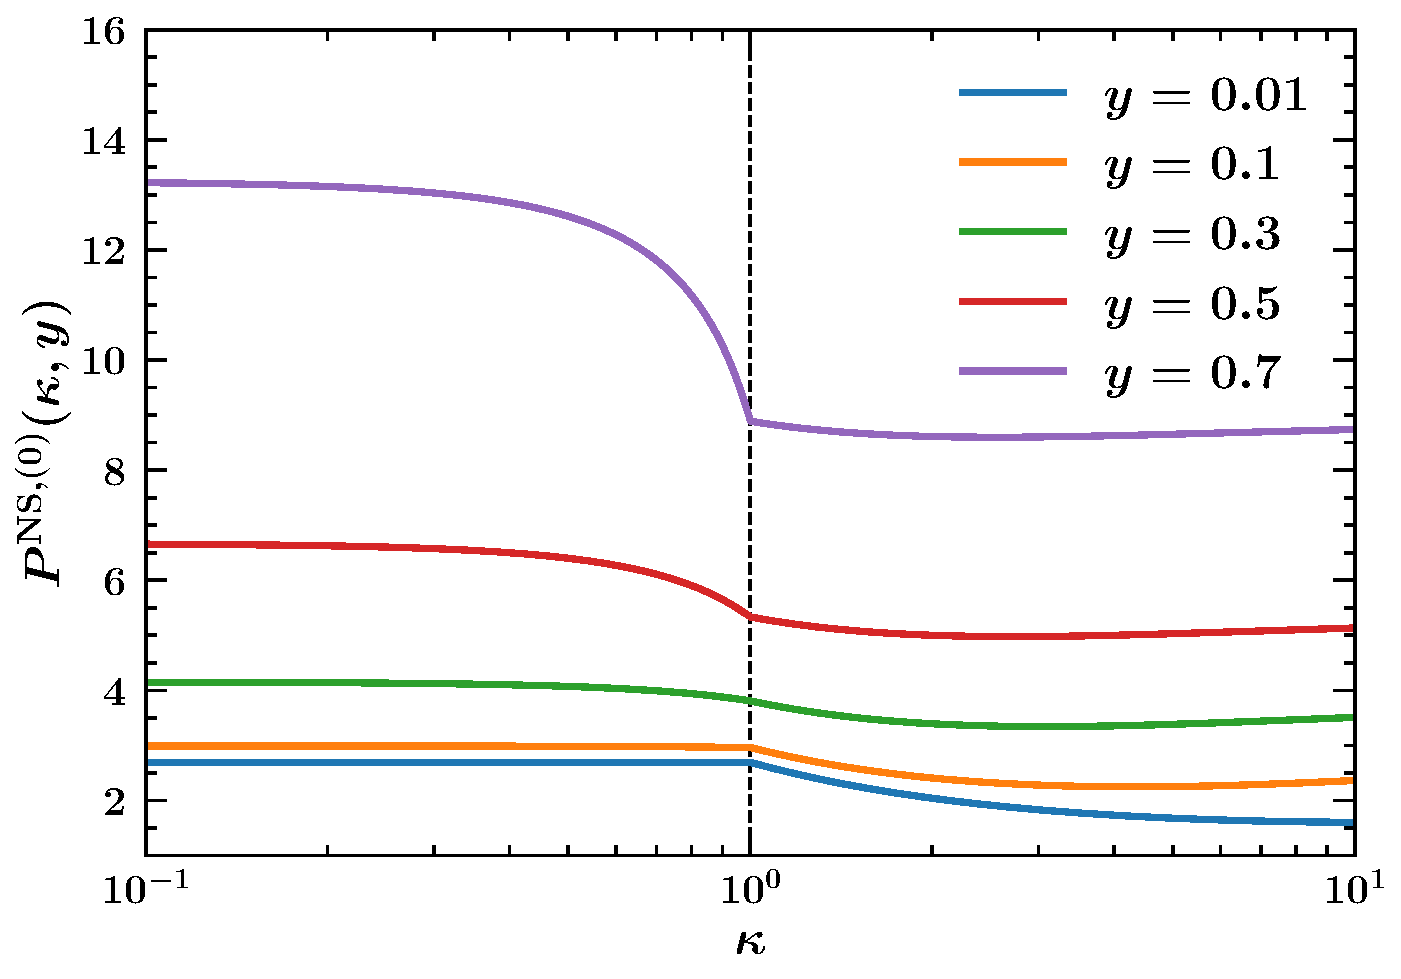
\includegraphics[width=0.6\textwidth]{plots/GPDP0}
    \caption{Behaviour of the anomalous dimension
      $P^{{\rm NS},(0)}$ as a function of $\kappa$ for
      different values of $y$.\label{fig:GPDP0}}
  \end{centering}
\end{figure}
Since $P_{qq}^{(0)}=P^{{\rm NS},(0)}$, what we discussed above applies
verbatim to $P_{qq}^{(0)}$.

Let us now turn to the remaining splitting functions $P_{qg}^{(0)}$,
$P_{gq}^{(0)}$, and $P_{gg}^{(0)}$. Their explicit expressions
read\footnote{The expression for $P_{gq}^{(0)}$ derived from
  Ref.~\cite{Blumlein:1999sc} seems to be wrong. I have derived the
  seemingly correct expression from Ref.~\cite{Ji:1996nm} by
  performing the replacement $\xi\rightarrow 2\kappa y$ in Eq.~(24).}:
\begin{equation}\label{eq:GPDP0qg}
  P_{qg}^{(0)}(\kappa,y) =\left\{
\begin{array}{ll}
  \displaystyle
  4 n_f T_R \frac{1 - 2y + (2 - \kappa^2) y^2}{(1 - \kappa^2 y^2)^2}\,,&\quad
                                                                 0\leq\kappa\leq
                                                                 1\,,\\
  \\
  \displaystyle 2n_f T_R \left[\frac{1 + \kappa}{\kappa^2 (1 + \kappa y)}\right] \left[\frac{1 - \kappa}{\kappa y }+\frac{1}{1 + \kappa y}\right]\,,&\displaystyle \quad 1
                                   \leq\kappa\leq\frac{1}{x}\,,
\end{array}
\right.
\end{equation}
\begin{equation}\label{eq:GPDP0gq}
  P_{gq}^{(0)}(\kappa,y) =\left\{
\begin{array}{ll}
  \displaystyle
2 C_F \left[\frac{2 - 2y + (1 - \kappa^2) y^2}{y (1 - \kappa^2 y^2)}\right]\,,&\quad
                                                                 0\leq\kappa\leq
                                                                 1\,,\\
  \\
\displaystyle  C_F \left[\frac{2(1+\kappa) - (1 - \kappa^2) y}{\kappa y (1 + \kappa y)}\right]\,,&\displaystyle \quad 1
                                   \leq\kappa\leq\frac{1}{x}\,,
\end{array}
\right.
\end{equation}
\begin{equation}\label{eq:GPDP0gg}
  P_{gg}^{(0)}(\kappa,y) =\left\{
\begin{array}{ll}
  \displaystyle
4 C_A\left[ \frac{-2 + y (1 - y + \kappa^2 (1 + y))}{(1 - \kappa^2 y^2)^2}+\frac{1}{y}+\frac1{\left(1-y\right)_+}\right]+\delta(1-x)\frac{11C_A-4n_fT_R}{3}\,,&\quad
                                                                 0\leq\kappa\leq
                                                                 1\,,\\
  \\
\displaystyle  C_A\left[\frac{-1 + 3 \kappa^2 - 
   \kappa (2 + (1 - \kappa)^2 \kappa) y}{\kappa^3 y (1 + \kappa y)^2}+\frac{2}{y}+\frac{2}{\left(1-y\right)_+}\right]+\delta(1-x)\frac{11C_A-4n_fT_R}{3}
\,,&\displaystyle \quad 1
                                   \leq\kappa\leq\frac{1}{x}\,.
\end{array}
\right.
\end{equation}
Their forward limit ($\kappa=0$) is:
\begin{equation}
\begin{array}{l}
  \displaystyle P_{qg}^{(0)}(0,y) = 4 n_f T_R \left[y^2+(1 - y)^2\right] \\
\\
  \displaystyle
P_{gq}^{(0)}(0,y) =2 C_F \left[\frac{1+(1 - y)^2}{y}\right]\,,\\
\\
  \displaystyle
  P_{gg}^{(0)}(0,y) =4 C_A\left[ -2 + y (1 - y)+\frac{1}{y}+\frac1{\left(1-y\right)_+}\right]+\delta(1-x)\frac{11C_A-4n_fT_R}{3}\,,
\end{array}
\end{equation}
which coincides with the usual one-loop DGLAP splitting functions. At
the crossover point $\kappa=1$ the evolution kernels reduce to:
\begin{equation}
  P_{qg}^{(0)}(1,y) = \frac{4 n_f T_R}{(1 + y)^2}\,,
\end{equation}
\begin{equation}
  P_{gq}^{(0)}(1,y) =\frac{4 C_F}{y (1 + y)}\,,
\end{equation}
\begin{equation}
  P_{gg}^{(0)}(1,y) =4 C_A\left[\frac{1+y^2}{y(1 + y)^2 \left(1-y\right)_+}\right]+\delta(1-y)\frac{11C_A-4n_fT_R}{3}\,.
\end{equation}
Interestingly, like $P^{{\rm NS},(0)}$ and $P_{qq}^{(0)}$ , also
$P_{qg}^{(0)}$, $P_{gq}^{(0)}$, and $P_{gg}^{(0)}$ are continuos in
$\kappa=1$.





\newpage
\appendix

\section{On Vinnikov's code}

The purpose of this Appendix is to draw the attention on a possible
incongruence of the GPD evolution code developed by Vinnikov and
presented in Ref.~\cite{Vinnikov:2006xw}. For definiteness, we
concentrate on the non-singlet $H_{\rm NS}$ GPD in the DGLAP region
$x>\xi$, whose evolution equation is given in Eq.~(29). For
completeness, I report that equation here:
\begin{equation}\label{eq:Vinnikov}
\begin{array}{rcl}
\displaystyle \frac{d H_{\rm NS}(x,\xi,Q^2)}{d\ln
  Q^2}&=&\displaystyle\frac{2\alpha_s(Q^2)}{3\pi}\Bigg[\int_x^1 dy
          \frac{x^2+y^2-2\xi^2}{(y-x)(y^2-\xi^2)}\left(H_{\rm
          NS}(y,\xi,Q^2)-H_{\rm NS}(x,\xi,Q^2)\right)\\
\\
&+&\displaystyle H_{\rm
    NS}(x,\xi,Q^2)\bigg(\frac32+2\ln(1-x)+\frac{x-\xi}{2\xi}\ln((x-\xi)(1+\xi))\\
\\
&-&\displaystyle \frac{x+\xi}{2\xi}\ln((x+\xi)(1-\xi))\bigg)\Bigg]\,.
\end{array}
\end{equation}
The limit for $\xi\rightarrow 0$ of the equation above should
reproduce the usual DGLAP evolution equation:
\begin{equation}
\displaystyle \frac{d H_{\rm 
NS}(x,0,Q^2)}{d\ln
  Q^2}=\frac{\alpha_s(Q^2)}{4\pi}\int_x^1 \frac{dz}{z}\left[\hat{P}_{\rm
  NS}\left(z\right)\right]_+H_{\rm NS}\left(\frac{x}{z},0,Q^2\right)\,,
\end{equation}
where:
\begin{equation}
\hat{P}_{\rm NS}\left(z\right)=2C_F\frac{1+z^2}{1-z}=2C_F\left[\frac{2}{1-z}-(1+z)\right]\,,
\end{equation}
with $C_F=4/3$. Written explicitly:
\begin{equation}\label{eq:DGLAPexpl}
\begin{array}{rcl}
  \displaystyle \frac{d H_{\rm NS}(x,0,Q^2)}{d\ln
    Q^2}&=&\displaystyle \frac{\alpha_s(Q^2)}{4\pi}2C_F\Bigg[\int_x^1 dz\,\frac{2}{1-z}\left(\frac1z H_{\rm NS}\left(\frac{x}{z},0,Q^2\right)-H_{\rm
      NS}(x,0,Q^2)\right)\\
\\
&-&\displaystyle \int_x^1 \frac{dz}{z}\, (1+z) H_{\rm
    NS}\left(\frac{x}{z},0,Q^2\right)\\
\\
 &+&\displaystyle H_{\rm NS}(x,0,Q^2)\left(\frac{3}{2}+2\ln(1-x)\right)\Bigg]\,.
\end{array}
\end{equation}
Now I explicitly take the limit for $\xi\rightarrow 0$ of
Eq.~(\ref{eq:Vinnikov}). The result is:
\begin{equation}
\begin{array}{rcl}
\displaystyle \frac{d H_{\rm NS}(x,0,Q^2)}{d\ln
  Q^2}&=&\displaystyle\frac{2\alpha_s(Q^2)}{3\pi}\Bigg[\int_x^1 dy
          \frac{x^2+y^2}{y^2 (y-x)}\left(H_{\rm
          NS}(y,0,Q^2)-H_{\rm NS}(x,0,Q^2)\right)\\
\\
&+&\displaystyle H_{\rm
    NS}(x,0,Q^2)\left(\frac32+2\ln(1-x)\right)\Bigg]\,.
\end{array}
\end{equation}
Some further simple algebraic manipulation finally gives:
\begin{equation}
\begin{array}{rcl}
\displaystyle \frac{d H_{\rm NS}(x,0,Q^2)}{d\ln
  Q^2}&=&\displaystyle\frac{\alpha_s(Q^2)}{4\pi}2C_F\Bigg[\int_x^1 dz\, 
          \frac{2}{1-z}\left(\frac{1}{z}H_{\rm
          NS}\left(\frac{x}{z},0,Q^2\right)-H_{\rm NS}(x,0,Q^2)\right)\\
\\
&-&\displaystyle \int_x^1 \frac{dz}{z}\,(1+z)H_{\rm
          NS}\left(\frac{x}{z},0,Q^2\right)\\
\\
&+&\displaystyle H_{\rm
    NS}(x,0,Q^2) \left(\frac32+2\ln(1-x)+\ln(x)+(1-x)\right)\Bigg]\,,
\end{array}
\end{equation}
that is close to the correct results, Eq.~(\ref{eq:DGLAPexpl}), except
for the two additional terms in the third line. Since the
$\xi\rightarrow 0$ limit does not seem to produce the correct result,
this suggests that the evolution code presented in
Ref.~\cite{Vinnikov:2006xw} may not be entirely correct.\footnote{It
  is, in fact, possible to correct Eq.~(\ref{eq:Vinnikov}) in such a
  way that its $\xi\rightarrow 0$ limit gives the correct DGLAP
  evolution equation.}

\newpage

\begin{thebibliography}{alp}

%\cite{Diehl:2003ny}
\bibitem{Diehl:2003ny}
  M.~Diehl,
  %``Generalized parton distributions,''
  Phys.\ Rept.\  {\bf 388} (2003) 41
  doi:10.1016/j.physrep.2003.08.002, 10.3204/DESY-THESIS-2003-018
  [hep-ph/0307382].
  %%CITATION = doi:10.1016/j.physrep.2003.08.002, 10.3204/DESY-THESIS-2003-018;%%
  %1016 citations counted in INSPIRE as of 30 Oct 2019

%\cite{Blumlein:1999sc}
\bibitem{Blumlein:1999sc}
  J.~Blumlein, B.~Geyer and D.~Robaschik,
  %``The Virtual Compton amplitude in the generalized Bjorken region: twist-2 contributions,''
  Nucl.\ Phys.\ B {\bf 560} (1999) 283
  doi:10.1016/S0550-3213(99)00418-6
  [hep-ph/9903520].
  %%CITATION = doi:10.1016/S0550-3213(99)00418-6;%%
  %86 citations counted in INSPIRE as of 13 Feb 2020

%\cite{Radyushkin:1997ki}
\bibitem{Radyushkin:1997ki}
A.~V.~Radyushkin,
%``Nonforward parton distributions,''
Phys. Rev. D \textbf{56} (1997), 5524-5557
doi:10.1103/PhysRevD.56.5524
[arXiv:hep-ph/9704207 [hep-ph]].
%1104 citations counted in INSPIRE as of 02 Jul 2020

%\cite{Ji:1996nm}
\bibitem{Ji:1996nm}
X.~D.~Ji,
%``Deeply virtual Compton scattering,''
Phys. Rev. D \textbf{55} (1997), 7114-7125
doi:10.1103/PhysRevD.55.7114
[arXiv:hep-ph/9609381 [hep-ph]].
%1183 citations counted in INSPIRE as of 08 Jul 2020

%\cite{Vinnikov:2006xw}
\bibitem{Vinnikov:2006xw}
A.~V.~Vinnikov,
%``Code for prompt numerical computation of the leading order GPD evolution,''
[arXiv:hep-ph/0604248 [hep-ph]].
%21 citations counted in INSPIRE as of 20 Jul 2020

\end{thebibliography}

\end{document}
